\DiaryEntry{Elevator Problem}{2015-12-15}{Maths}

\subsection{Elevator Problem, allowing multiple selection of the same
Floor}

Consider an elevator stopping at $n$ different floors. There are $k$ people using the elevator and every person selects a floor by pressing a button. The selection of $k$ floors (by $k$ people) is denoted as $(f_1,f_2,\cdots,f_k) $ where $f_i$ is the floor selected by the $i$-th person. Different people may select the same floor; i.e.~sequences like $(1,1,3)$ are allowed.

What is the probability that $k$ consecutive floors are selected (e.g. (1,2,3) or (4,5,6)?

First, note that we count (1,2,3) and (3,1,2) as two different sequences.

With this assumption, there are $n^k$ possibilities to press $k$ buttons out of $n$.

In order to count the number of ``good'' cases (i.e.~consecutive floors), assume that the first $k$ floors are pressed; i.e.~we have $ (1,2,\ldots,k) $. The order of the buttons does not matter, so we can arrange the sequence in $k!$ different ways (k possibilities for the first element, k-1 for the second and so on). E.g. for $k=3$ we have (1,2,3), (2,1,3), (3,2,1), (2,3,1), (3,1,2), and (1,3,2).

The first set has the form $1,2,\ldots,k$, the second has the form $(2,3,\ldots,k+1)$, and the last set $(n-k+1,n-k+2,\ldots,n)$. In total we have $n-k+1$ sets. E.g. for $k=3$ and $n=5$, we have $(1,2,3)$, $(2,3,4)$, $(3,4,5)$.

So the total number of ``good'' cases is $k!(n-k+1)$ and therefore the probability that $k$ consecutive buttons are pressed is

\[
P = \frac{k!(n-k+1)}{n^k}
\]

The Figure below show the probability for $n=13$ as a function of $k$. For $k=1$ it is $1$, as any sequence of length 1 is consecutive. For larger $k$, the probability decreases quickly.

\begin{figure}[H]
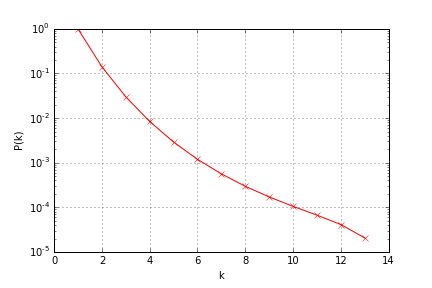
\includegraphics[scale=0.7]{images/elevator.png}
\end{figure}

The Figure below show the probability for $k=10$ as a function of $n$. The probability decreases quickly.

\begin{figure}
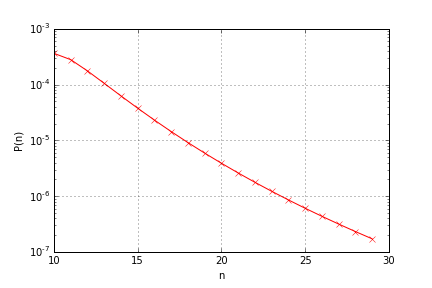
\includegraphics[scale=0.7]{images/elevator_2.png}
\end{figure}

\subsubsection{Additional}

The probability expression above leads to the question how a function

\[
f(k) = \frac{k!}{n^k}
\]

behaves. A plot of the function for $n=10$ (red) and for $n=15$ (blue) is shown below.

\begin{figure}
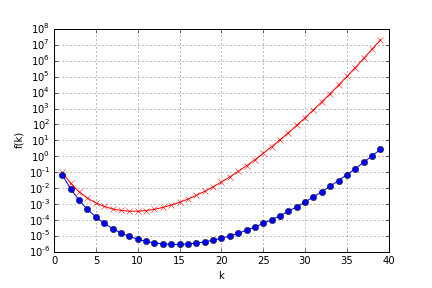
\includegraphics[scale=0.7]{images/factorial_vs_exp.png}
\end{figure}

We first inspect the interesting point $k=n$: We have $f(n) = \frac{n!}{n^n}$. The point to the left, $k=n-1$ yields the following interesting value:

\[
f(n-1) = \frac{(n-1)!}{n^{n-1}} = \frac{(n-1)! n }{n^{n-1} n } = \frac{n!}{n^{n}} = f(n)
\]

Nice :-)

Going further to the left, we have for positive $l$

\[
\frac{f(n-l)}{f(n-l+1)} = \frac{ \frac{(n-l)!}{n^{n-l}} }{ \frac{(n-l+1)!}{n^{n-l+1}} } = \frac{  (n-l)! n^{n-l+1}  }{ (n-l+1)! n^{n-l} } = \frac{n^{n-l+1-(n-l)}}{n-l+1} = \frac{n}{n-l+1} > 1, \, l > 1
\]

which proves that $f(k)$ is larger than $f(n)$ for $k\textless{}n-1$.

A similar argument can be made for points right of $n$. Here we have:

\[
\frac{f(n+l)}{f(n+l+1)} = \frac{ \frac{(n+l)!}{n^{n+l}} }{ \frac{(n+l+1)!}{n^{n+l+1}} } = \frac{  (n+l)! n^{n+l+1}  }{ (n+l+1)! n^{n+l} } = \frac{n^{n+l+1-(n+l)}}{n+l+1} = \frac{n}{n+l+1} < 1, \, l \geq 1
\]

which proves that $f(k)$ is larger than $f(n)$ for $k>n$.

This is the (more) interesting part - for large enough $k$, $k!$ grows larger than $n^k$.

\subsection{Elevator Problem, single selection of the same Floor}

In case we do not allow the selection of the same floor (button) by
different people, the only thing that changes is the total number of
cases: Before we had \(n^k\) (as all \(k\) persons were allowed to press one of the \(n\) floors), now after the first person has chosen one of the \(n\) floors, the second one has only \(n-1\) possibilities left and so on. So in total there are \(n \times (n-1) \times \cdots \times (n-k+1)\) possibilities. We can rewrite this as \(n!(n-k)!\) and so the probability becomes

\[
P^\star = \frac{k!(n-k+1)}{n!/(n-k)!}
\]

Comparing the two probabilities, we see that \(n^k\) is always larger
than \(n!/(n-k)!\) (in the first case we multiply n k-times; in the
second one, the first factor is n, then n-1 and so on). The nominator is the same, therefore, the probability \(p^\star\) is larger than \(P\). This makes sense, as allowing only single selection of the same floor results in a smaller number of total cases.

As an interesting sidenote (regarding simulation), it is only possible to have less persons than floors, i.e. \(k \leq n\) - otherwise not all persons cannot press different floors.
